\documentclass[12pt,a4paper,twoside]{report}
\usepackage[a4paper,outer=1cm,inner=3cm,top=2cm,bottom=1cm]{geometry}
\usepackage{setspace}
\usepackage{polyglossia}
\usepackage{fontspec}
\usepackage{xltxtra}
\usepackage{listings}
\usepackage{titlesec}
\usepackage{color}
\usepackage{xcolor}

\defaultfontfeatures{Scale=MatchLowercase}
\setsansfont[Mapping=tex-text]{Helvetica}
\renewcommand*{\familydefault}{\sfdefault}

\usepackage{amsmath}
\usepackage{amsfonts}

\titleformat{\section}{\normalfont\fontsize{25}{25}\bfseries\centering}{\thesection}{1em}{}
\newcommand{\sectionbreak}{\clearpage}

\title{
	Компьютерный праткикум по\\
	линейной алгебре.\\
	Расчётное задание №1\\[4em]
	\large {
		Тема: Матрицы и операции над ними.\\
		Обратная матрица. Системы векторов.\\
		Линейная зависимость и независимость.\\
		Системы линейных уравнений. \\
		Метод Гаусса. Ранг и база системы векторов.\\[4em]
	}
}
\author{Вилков Кирилл Олегович, группа 14ПИ}
\date{05.10.14}

\makeatletter
\def\Title{Расчётное задание №1}
\let\theauthor\@author
\makeatother

\usepackage{fancyhdr}
\pagestyle{fancy}
\fancyhf{}
\fancyhead[LE,RO]{\thepage}
\fancyhead[RE,LO]{\Title \qquad \theauthor}
\fancyheadoffset{0mm}
\fancyfootoffset{0mm}
\setlength{\headheight}{15pt}
\renewcommand{\headrulewidth}{1pt}
\renewcommand{\footrulewidth}{0pt}

\usepackage{tocloft}

\setcounter{tocdepth}{1}
\setcounter{secnumdepth}{0}
\renewcommand\contentsname{Содержание}
\tocloftpagestyle{fancy}

\usepackage{listings}
%\usepackage{courier}

\definecolor{dkgreen}{rgb}{0,0.6,0}
\definecolor{gray}{rgb}{0.5,0.5,0.5}
\definecolor{mauve}{rgb}{0.58,0,0.82}

\lstset{
	frame=tb,
	xleftmargin=20pt,
	language=Matlab,
	aboveskip=3mm,
	belowskip=3mm,
	showstringspaces=false,
	columns=flexible,
	basicstyle={\small\ttfamily},
	numbers=none,
	breaklines=true,
	breakatwhitespace=true
	tabsize=2
}

\newcommand{\showcode}[1]{
	%\begin{minipage}{\linewidth}
		\lstinputlisting{#1}
	%\end{minipage}
}
\newcommand{\showscreen}[1]{
\\ \includegraphics[scale=0.6]{#1} \\
}


\begin{document}

	\maketitle
	\pagestyle{fancy}
	\setcounter{page}{1}
	\tableofcontents
	\newpage

	\renewcommand*{\arraystretch}{1.5}

	\section{Задача 1.24}
\subsection{Задание:}
Решить
$
	\left|
		\begin{matrix}
			2 & x & 6 \\
			3 & 3 & 9 \\
			7 & 4 & 11
		\end{matrix}
	\right|
	= 0
$
\subsection{Решение:}
$
	3 \cdot 11 \cdot x + 2 \cdot 4 \cdot 9 + 2 \cdot 3 \cdot 11 -
	6 \cdot 3 \cdot 4 - 6 \cdot 3 \cdot 7 - 7 \cdot 9 \cdot x = 0
	\\[1ex]
	-30x - 60 = 0
	\\[1ex]
	x = -\dfrac{60}{30} = 2
$
\subsection{Проверим результат в среде Wolfram Mathematica:}
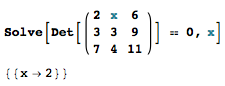
\includegraphics[scale=0.6]{task/1_24/screen.png}
\subsection{Ответ:}
Компьютерная проверка подтвердила полученный результат.

	\section{Задача 1.25}
\subsection{Задание:}
Найти матрицу обратную к
$
	A =
	\begin{pmatrix}
		2 & 4 & 0 & 1 \\
		3 & -3 & 5 & 0 \\
		-1 & 0 & 1 & 1 \\
		2 & 1 & 1 & 0 \\
	\end{pmatrix}
$
\; методом алгебраических дополненй.
\subsection{Решение:}
Найдём $ \det A $ чтобы убедиться что $ \exists A^{-1} $:
\\[1em]
$
	\det A =
	\begin{vmatrix}
		2 & 4 & 0 & 1 \\
		3 & -3 & 5 & 0 \\
		-1 & 0 & 1 & 1 \\
		2 & 1 & 1 & 0 \\
	\end{vmatrix}
	=
	\begin{vmatrix}
		3 & 4 & -1 & 0 \\
		3 & -3 & 5 & 0 \\
		-1 & 0 & 1 & 1 \\
		2 & 1 & 1 & 0 \\
	\end{vmatrix}
	=
	\begin{vmatrix}
		3 & 4 & -1 & 0 \\
		3 & -3 & 5 & 0 \\
		-1 & 0 & 1 & 1 \\
		2 & 1 & 1 & 0 \\
	\end{vmatrix}
	=
	-
	\begin{vmatrix}
		3 & 4 & -1 \\
		3 & -3 & 5 \\
		2 & 1 & 1 \\
	\end{vmatrix}
	=
	5
$
\\[1em]
$ \det A \neq 0 \Rightarrow \exists A^{-1} = \dfrac{D^T}{\det A} $
\\[1em]
$
	d_{11} =
	\begin{vmatrix}
		-3 & 5 & 0 \\
		0 & 1 & 1 \\
		1 & 1 & 0 \\
	\end{vmatrix}
	=
	\begin{vmatrix}
		-3 & 5 & 0 \\
		0 & 1 & 1 \\
		1 & 1 & 0 \\
	\end{vmatrix}
	=
	-
	\begin{vmatrix}
		-3 & 5 \\
		1 & 1 \\
	\end{vmatrix}
	= 8
\\[1em]
	d_{12} =
	\begin{vmatrix}
		3 & 5 & 0 \\
		-1 & 1 & 1 \\
		2 & 1 & 0 \\
	\end{vmatrix}
	=
	-
	\begin{vmatrix}
		3 & 5 \\
		2 & 1 \\
	\end{vmatrix}
	=
	7
\\[1em]
	d_{13} =
	\begin{vmatrix}
		3 & -3 & 0 \\
		-1 & 0 & 1 \\
		2 & 1 & 0 \\
	\end{vmatrix}
	=
	-
	\begin{vmatrix}
		3 & -3 \\
		2 & 1 \\
	\end{vmatrix}
	=
	-9
\\[1em]
	d_{14} =
	\begin{vmatrix}
		3 & -3 & 5 \\
		-1 & 0 & 1 \\
		2 & 1 & 1 \\
	\end{vmatrix}
	=
	\begin{vmatrix}
		-3 & 5 \\
		1 & 1 \\
	\end{vmatrix}
	-
	\begin{vmatrix}
		3 & -3 \\
		2 & 1 \\
	\end{vmatrix}
	=
	-8 - 9 = -17
\\[1em]
	d_{21} =
	\begin{vmatrix}
		4 & 0 & 1 \\
		0 & 1 & 1 \\
		1 & 1 & 0 \\
	\end{vmatrix}
	=
	4
	\begin{vmatrix}
		1 & 1 \\
		1 & 0
	\end{vmatrix}
	+
	\begin{vmatrix}
		0 & 1 \\
		1 & 1
	\end{vmatrix}
	= -4 - 1 = -5
\\[1em]
	d_{22} =
	\begin{vmatrix}
		2  & 0 & 1 \\
		-1 & 1 & 1 \\
		2 & 1 & 0 \\
	\end{vmatrix}
	=
	2
	\begin{vmatrix}
		1 & 1 \\
		1 & 0 \\
	\end{vmatrix}
	+
	\begin{vmatrix}
		-1 & 1 \\
		2 & 1 \\
	\end{vmatrix}
	= -2 - 3 = -5
\\[1em]
$


\end{document}
